
% This LaTeX was auto-generated from MATLAB code.
% To make changes, update the MATLAB code and republish this document.

\documentclass{article}
\usepackage{graphicx}
\usepackage{color}

\sloppy
\definecolor{lightgray}{gray}{0.5}
\setlength{\parindent}{0pt}

\begin{document}

    
    

\section*{21. Spectral methods}

\begin{verbatim}
ATAPformats
\end{verbatim}
\begin{par}
Theorem 8.2 described the geometric convergence of Chebyshev projections and interpolants for an analytic function $f$ defined on $[-1,1]$.  For such a function, it is not just the polynomials that converge geometrically, but also their derivatives.  The following theorem makes this precise. An early publication with a result along these lines is [Tadmor 1986].
\end{par} \vspace{1em}
\begin{par}

{\em{\bf Theorem 21.1. Geometric convergence of derivatives.}
Let a function $f$ be analytic in $[-1,1]$ and analytically continuable
to the closed Bernstein ellipse $\overline E_\rho$ for some $\rho>1$.
Then for each integer $\nu\ge 0$, the $\nu\kern .7pt$th derivatives of
the Chebyshev projections $f_n$ and interpolants $p_n$ satisfy as
$n\to\infty$
$$ \| f^{(\nu)}-f_n^{(\nu)}\| = O(\kern.7pt\rho^{-n}),
\quad\|f^{(\nu)}-p_n^{(\nu)}\| = O(\kern.7pt\rho^{-n}). \eqno (21.1) $$
}

\end{par} \vspace{1em}
\begin{par}
\vskip -2.5em
\end{par} \vspace{1em}
\begin{par}
\textit{Proof.}  Here is an outline, to be filled in in Exercise 21.1. If $f$ is analytic in the closed region $\overline E_\rho$, it is also analytic and bounded in the open region $E_{\tilde \rho}$ for some $\tilde \rho > \rho$. By Theorem 8.1 it follows that the Chebyshev coefficients satisfy $a_k = O(\kern .7pt \tilde \rho^{\,-k})$. The bounds (21.1) follow by differentiating the Chebyshev series  for $f^{(\nu)}-f_n^{(\nu)}$ and $f^{(\nu)}-p_n^{(\nu)}$ term by term.  The differentiations introduce powers of $n$, since $T_n'$ is of size $O(n^2)$ on $[-1,1]$, for example, but since $n^\alpha \tilde \rho^{\,-n} = O(\kern.7pt\rho^{-n})$ as $n\to\infty$ for any fixed $\alpha$, we still get $O(\kern.7pt\rho^{-n})$ convergence for any fixed $\nu$. $~\hbox{\vrule width 2.5pt depth 2.5 pt height 3.5 pt}$
\end{par} \vspace{1em}
\begin{par}

The phenomenon captured in Theorems 8.2 and 21.1 is a general one in
complex analysis.  When a property holds for an analytic function, there is
a good chance that a similar property holds for its derivatives too.  The
ultimate reason is that both function and derivative can be related to
Cauchy integrals, and indeed, an alternative proof of
Theorem 21.1 can be based on the Hermite integral formula.

\end{par} \vspace{1em}
\begin{par}
The present chapter is a practical one, devoted to outlining some of the wide-ranging consequences of Theorem 21.1 for scientific computing: the whole field of \textit{spectral methods} for the numerical solution of differential equations. Spectral methods are noted for achieving \textit{spectral accuracy,} which means accuracy that is limited not by the order of the numerical discretization, but only by the smoothness of the function being approximated.  This is in contrast to a traditional finite difference or finite element method, which might achieve just $O((\Delta x)^2)$ or $O((\Delta x)^4)$ accuracy as $\Delta x \to 0$, say, where $\Delta x$ is a grid spacing, even when the function being approximated is $C^\infty$ or analytic. For a leisurely introduction to spectral methods on Chebyshev grids, see [Trefethen 2000].
\end{par} \vspace{1em}
\begin{par}
We now put aside $\{f_n\}$ and focus on \textit{spectral collocation methods,} based on point values and polynomial interpolants, as opposed to \textit{spectral Galerkin methods,} based on integrals.
\end{par} \vspace{1em}
\begin{par}

The starting point of spectral collocation methods is the notion of a
{\em differentiation matrix}.  If $p$ is a polynomial of degree $n$, it is
determined by its values on an $(n+1)$-point grid in $[-1,1]$.
The derivative $p'$, a polynomial of degree $n-1$, is determined by its
values on the same grid. The classical spectral differentiation matrix
is the $(n+1)\times (n+1)$ matrix that
represents the linear map from the vector of values of $p$ on the grid to
the vector of values of $p'$.
(Later we shall mention rectangular
alternatives to this classical square matrix formulation.)
An explicit formula for this matrix
follows from equation (5.8) and was first published
by Bellman, Kashev and Casti [1972] (Exercise 21.9):
$$ D_{ij} = \ell_j'(x_i) = \cases{
\displaystyle{\lambda_j\over \lambda_i (x_i-x_j)} & $i \ne j$, \cr
\noalign{\vskip 5pt}
\displaystyle{x_j\over 1-x_j^2} & $i=j$.} \eqno (21.2) $$

\end{par} \vspace{1em}
\begin{par}
The particularly important special case is that of a Chebyshev grid. For example, the function $\sin(x)$ can be represented to machine precision by a Chebyshev interpolant $p$ on a grid of 14 points:
\end{par} \vspace{1em}
\begin{par}
 \vskip -2em 
\end{par} \vspace{1em}
\begin{verbatim}
x = chebfun('x'); p = sin(x); length(p)
\end{verbatim}

        \color{lightgray} \begin{verbatim}ans =
    14
\end{verbatim} \color{black}
    \begin{par}
Suppose we wish to calculate the values of $p'$ on the same grid. In Chebfun we can write
\end{par} \vspace{1em}
\begin{par}
 \vskip -2em 
\end{par} \vspace{1em}
\begin{verbatim}
pp = diff(p); x14 = chebpts(14); pp14 = pp(x14)
\end{verbatim}

        \color{lightgray} \begin{verbatim}pp14 =
   0.540302305868161
   0.564522388819888
   0.632936510563863
   0.732703188872980
   0.842943722651217
   0.937783753082982
   0.992744245701781
   0.992744245701781
   0.937783753082982
   0.842943722651217
   0.732703188872980
   0.632936510563863
   0.564522388819888
   0.540302305868161
\end{verbatim} \color{black}
    \begin{par}
But we can also get our hands on the differentiation matrix explicitly with these commands involving a chebfun object known as a ``chebop'':
\end{par} \vspace{1em}
\begin{par}
 \vskip -2em 
\end{par} \vspace{1em}
\begin{verbatim}
D = chebop(@(u) diff(u)); D14 = D(14);
\end{verbatim}
\begin{par}
If the matrix \texttt{D14} is multiplied by the vector \texttt{p(x14)}, the result is the same vector \texttt{pp14} of sampled derivatives, up to rounding errors:
\end{par} \vspace{1em}
\begin{par}
 \vskip -2em 
\end{par} \vspace{1em}
\begin{verbatim}
norm(pp14-D14*p(x14))
\end{verbatim}

        \color{lightgray} \begin{verbatim}ans =
     4.048114308080452e-14
\end{verbatim} \color{black}
    \begin{par}
Above, we put a semicolon after \texttt{D(14)} to avoid printing a $14\times 14$ matrix.  To give the idea while using up a little less space, here are the $3\times 3$ and $5\times 5$ Chebyshev differentiation matrices on $[-1,1]$:
\end{par} \vspace{1em}
\begin{par}
 \vskip -2em 
\end{par} \vspace{1em}
\begin{verbatim}
format short, D(3)
\end{verbatim}

        \color{lightgray} \begin{verbatim}ans =
   -1.5000    2.0000   -0.5000
   -0.5000         0    0.5000
    0.5000   -2.0000    1.5000
\end{verbatim} \color{black}
    \begin{par}
 \vskip -2em 
\end{par} \vspace{1em}
\begin{verbatim}
D(5)
\end{verbatim}

        \color{lightgray} \begin{verbatim}ans =
   -5.5000    6.8284   -2.0000    1.1716   -0.5000
   -1.7071    0.7071    1.4142   -0.7071    0.2929
    0.5000   -1.4142    0.0000    1.4142   -0.5000
   -0.2929    0.7071   -1.4142   -0.7071    1.7071
    0.5000   -1.1716    2.0000   -6.8284    5.5000
\end{verbatim} \color{black}
    \begin{par}
Formulas for the entries of Chebyshev differentiation matrices were first published by Gottlieb, Hussaini \& Orszag [1984], and recurrence relations for computing them fast and stably were given by Welfert [1997], based on earlier work by Fornberg [1988].  Welfert's paper in turn led to the influential Matlab Differentiation Matrix Suite by Weideman and Reddy [2000], and another Matlab code \texttt{cheb} for generating these matrices can be found in [Trefethen 2000].
\end{par} \vspace{1em}
\begin{par}
There is no need to stop at the first derivative. Here is the $5\times 5$ Chebyshev matrix corresponding to the second derivative on $[-1,1]$:
\end{par} \vspace{1em}
\begin{par}
 \vskip -2em 
\end{par} \vspace{1em}
\begin{verbatim}
D2 = chebop(@(u) diff(u,2)); D2(5)
\end{verbatim}

        \color{lightgray} \begin{verbatim}ans =
   17.0000  -28.4853   18.0000  -11.5147    5.0000
    9.2426  -14.0000    6.0000   -2.0000    0.7574
   -1.0000    4.0000   -6.0000    4.0000   -1.0000
    0.7574   -2.0000    6.0000  -14.0000    9.2426
    5.0000  -11.5147   18.0000  -28.4853   17.0000
\end{verbatim} \color{black}
    \begin{par}
Yes, \texttt{D2(5)} is the square of \texttt{D(5)}:
\end{par} \vspace{1em}
\begin{par}
 \vskip -2em 
\end{par} \vspace{1em}
\begin{verbatim}
norm(D2(5)-(D(5))^2)
\end{verbatim}

        \color{lightgray} \begin{verbatim}ans =
   9.1262e-14
\end{verbatim} \color{black}
    \begin{par}

The entries of this matrix can be interpreted as follows. The $j$th
column $(0 \le j \le n$) contains the second derivatives of the Lagrange
polynomial $\ell_j(x)$ evaluated at grid points $x_0,\dots, x_n$.  That
is, its $(i,j)$ entry (with indexing from $0$ to $n$) is $\ell_j''(x_i)$.
(We have seen Lagrange polynomials in Chapters 5, 9, 11, and 15.) For
example, here is the Lagrange polynomial supported at $x_3$:

\end{par} \vspace{1em}
\begin{par}
 \vskip -2em 
\end{par} \vspace{1em}
\begin{verbatim}
p3 = chebfun([0 0 0 1 0]'); FS = 'fontsize';
clf, plot(p3,'.-'), title('Lagrange polynomial l_3',FS,9)
\end{verbatim}

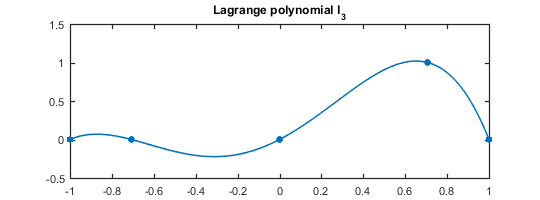
\includegraphics [width=4in]{chap21_01.png}
\begin{par}
 \vskip 1pt 
\end{par} \vspace{1em}
\begin{par}
Its second derivatives at the grid points are the values in the fourth column of the matrix $D(5)$ just shown:
\end{par} \vspace{1em}
\begin{par}
 \vskip -2em 
\end{par} \vspace{1em}
\begin{verbatim}
p3pp = diff(p3,2); x5 = chebpts(5); p3pp(x5)
\end{verbatim}

        \color{lightgray} \begin{verbatim}ans =
  -11.5147
   -2.0000
    4.0000
  -14.0000
  -28.4853
\end{verbatim} \color{black}
    \begin{par}

In Chebfun, an object like {\tt D} or {\tt D2} is called a {\em linear
chebop} (and internally within the Chebfun system, a {\em linop}).  A
linear chebop is not a matrix, but rather a prescription for how to
construct matrices of arbitrary order. (A computer science term for the
process of filling such prescriptions is {\em lazy evaluation}.) If $D$
is applied to an integer argument, the matrix of that dimension is
produced:

\end{par} \vspace{1em}
\begin{par}
 \vskip -2em 
\end{par} \vspace{1em}
\begin{verbatim}
size(D(33))
\end{verbatim}

        \color{lightgray} \begin{verbatim}ans =
    33    33
\end{verbatim} \color{black}
    \begin{par}
If $D$ is applied to a chebfun, it has the effect appropriate to the length of that chebfun:
\end{par} \vspace{1em}
\begin{par}
 \vskip -2em 
\end{par} \vspace{1em}
\begin{verbatim}
f = sin(7*x).*exp(x).*tan(x); norm(diff(f)-D*f)
\end{verbatim}

        \color{lightgray} \begin{verbatim}ans =
     0
\end{verbatim} \color{black}
    \begin{par}
More generally, a chebop can be defined for any differential (or integral) operator.  For example, here is the chebop corresponding to the map $L: u \mapsto u'' + u' + 100u$ on $[-1,1]$:
\end{par} \vspace{1em}
\begin{par}
 \vskip -2em 
\end{par} \vspace{1em}
\begin{verbatim}
L = chebop(@(u) diff(u,2) + diff(u) + 100*u);
\end{verbatim}
\begin{par}
Here is the $5\times 5$ realization of this operator:
\end{par} \vspace{1em}
\begin{par}
 \vskip -2em 
\end{par} \vspace{1em}
\begin{verbatim}
L(5)
\end{verbatim}

        \color{lightgray} \begin{verbatim}ans =
  111.5000  -21.6569   16.0000  -10.3431    4.5000
    7.5355   86.7071    7.4142   -2.7071    1.0503
   -0.5000    2.5858   94.0000    5.4142   -1.5000
    0.4645   -1.2929    4.5858   85.2929   10.9497
    5.5000  -12.6863   20.0000  -35.3137  122.5000
\end{verbatim} \color{black}
    \begin{par}
We can illustrate its use by applying it to the chebfun for $e^x$:
\end{par} \vspace{1em}
\begin{par}
 \vskip -2em 
\end{par} \vspace{1em}
\begin{verbatim}
f = exp(x); Lf = L*f;
Lfexact = 102.*exp(x); norm(Lf-Lfexact)
\end{verbatim}

        \color{lightgray} \begin{verbatim}ans =
   1.9992e-13
\end{verbatim} \color{black}
    \begin{par}
Now we come at last to spectral methods proper.  If we just wanted to apply differential operators to functions, we would not need matrices. To solve a differential equation, however, we need to invert the process of applying a differential operator. We want to find a function $u$ satisfying certain boundary conditions such that $Lu$ is equal to a prescribed function $f$.  This is where the matrices come in, for matrices can be inverted.
\end{par} \vspace{1em}
\begin{par}
Suppose, for example, we seek a function $u$ that satisfies the equation $$ u'' + u' + 100u = x , \quad u(-1) = u(1) = 0 \eqno (21.3) $$ with $x\in[-1,1]$. The matrix realization above had no boundary conditions.  Now we need to impose them, and a standard way of doing this is to modify one or more initial or final rows of the matrix, one row for each boundary condition (see Chapters 7 and 13 of [Trefethen 2000]). For Dirichlet boundary conditions as in (21.3), we change the first and last rows to correspond to rows of the identity:
\end{par} \vspace{1em}
\begin{par}
 \vskip -2em 
\end{par} \vspace{1em}
\begin{verbatim}
L.bc = 'dirichlet'; feval(L,5,'oldschool')
\end{verbatim}

        \color{lightgray} \begin{verbatim}ans =
    1.0000         0         0         0         0
    7.5355   86.7071    7.4142   -2.7071    1.0503
   -0.5000    2.5858   94.0000    5.4142   -1.5000
    0.4645   -1.2929    4.5858   85.2929   10.9497
         0         0         0         0    1.0000
\end{verbatim} \color{black}
    \begin{par}
(We shall explain the clumsy command \texttt{feval(L,5,'oldschool')} in a moment.) Thus, instead of imposing the differential equation at the boundary points $x_0$ and $x_n$, we are imposing boundary conditions at those points.  We can now use exactly this matrix to solve the ODE approximately with a $5\times 5$ spectral discretization.  The right-hand side of the matrix problem will be the vector of $x$ sampled at the Chebyshev points---except that the first and last components of the vector will be changed to the appropriate Dirichlet values at $x_0$ and $x_n$, namely zero.
\end{par} \vspace{1em}
\begin{par}
 \vskip -2em 
\end{par} \vspace{1em}
\begin{verbatim}
x5 = chebpts(5); x5([1 end]) = 0;
u5 = feval(L,5,'oldschool')\x5;
plot(chebfun(u5),'.-')
title('Spectral solution to (21.3) on 5-point grid',FS,9)
\end{verbatim}

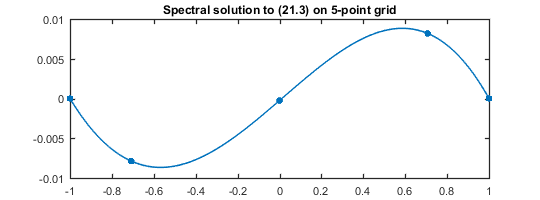
\includegraphics [width=4in]{chap21_02.png}
\begin{par}
 \vskip 1pt 
\end{par} \vspace{1em}
\begin{par}
We have just computed our first solution of a boundary value problem with a spectral method.  From the picture it is not evident whether the result is close to correct or not.  In fact it is not, as increasing the resolution reveals:
\end{par} \vspace{1em}
\begin{par}
 \vskip -2em 
\end{par} \vspace{1em}
\begin{verbatim}
x12 = chebpts(12); x12([1 end]) = 0;
u12 = feval(L,12,'oldschool')\x12;
plot(chebfun(u12),'.-')
title('Spectral solution to (21.3) on 12-point grid',FS,9)
\end{verbatim}

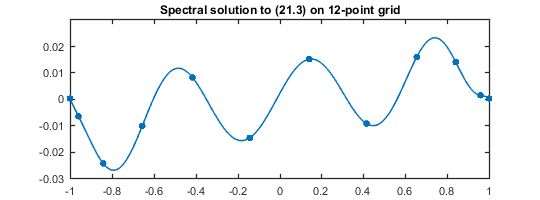
\includegraphics [width=4in]{chap21_03.png}
\begin{par}
 \vskip 1pt 
\end{par} \vspace{1em}
\begin{par}
This curve is beginning to get close to the true solution. How fine a grid do we need to reach approximately machine precision? In Chebfun, the appropriate grid is determined automatically when one solves the problem without specifying dimensions, still with the backslash command:
\end{par} \vspace{1em}
\begin{par}
 \vskip -2em 
\end{par} \vspace{1em}
\begin{verbatim}
u = L\x; plot(u,'.-')
title(['Spectral solution to (21.3) on ' ...
    'automatically determined grid'],FS,9)
\end{verbatim}

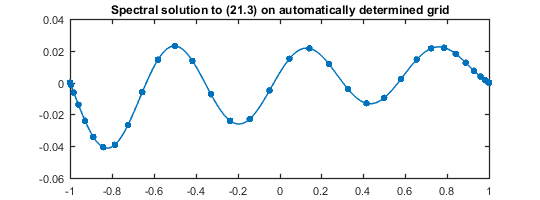
\includegraphics [width=4in]{chap21_04.png}
\begin{par}
 \vskip 1pt 
\end{par} \vspace{1em}
\begin{par}
To get this result, Chebfun has solved matrix problems of sizes $9$, $17$, $33$, and $65$, at which point it found that its convergence criteria were satisfied. The final length is
\end{par} \vspace{1em}
\begin{par}
 \vskip -2em 
\end{par} \vspace{1em}
\begin{verbatim}
length(u)
\end{verbatim}

        \color{lightgray} \begin{verbatim}ans =
    34
\end{verbatim} \color{black}
    \begin{par}
and we can verify that the accuracy is good:
\end{par} \vspace{1em}
\begin{par}
 \vskip -2em 
\end{par} \vspace{1em}
\begin{verbatim}
norm(L*u-x)
\end{verbatim}

        \color{lightgray} \begin{verbatim}ans =
   1.0766e-12
\end{verbatim} \color{black}
    \begin{par}

This brings us to the clumsy expression \verb|feval(L,5,'oldschool')| in
the demonstration above.  This notation instructs Chebfun to display a
spectral differentiation matrix corresponding to boundary conditions
imposed in the classical way that we have just described, in which
certain rows of a square differentiation matrix are replaced by rows
corresponding to boundary conditions [Trefethen 2000]. This method of
applying boundary conditions relies on the assumption that for each
boundary condition, there is a clear choice of which row of the ODE discretization
matrix it should replace. In fact, this ceases to be clear in
various situations involving systems of equations or more complicated
boundary conditions, as well as more general side conditions such as
$\int \kern -.7pt u(x) \kern .7pt dx = 0$.  Around 2010, Driscoll and
Hale realized that more robust and flexible discretizations could be
obtained by switching to a different approach based on rectangular
differentiation matrices. For an order $d$ differential operator to be
applied on an $(n+1)$-point grid, the Driscoll--Hale discretization
begins with a matrix of dimension $(n+1-d\kern 1pt )\times (n+1)$
corresponding to a map from data on an $(n+1)$-grid to data on an
$(n+1-d\kern 1pt )$-grid, and then appends an additional $d$ rows for
boundary conditions.  No collocation equation gets replaced in this
process. This is now the discretization strategy used routinely by
Chebfun, and it is what Chebfun actually did in solving the problem
\verb|u = L\x| above. To see the matrices, one can type the more natural
expression \verb|L(5)| instead of \verb|feval(L,5,'oldschool')|.  We
shall not go into details here; see [Driscoll \& Hale 2012].

\end{par} \vspace{1em}
\begin{par}
Homogeneous Dirichlet conditions at both ends are only the simplest of many possible boundary conditions for a boundary value problem.   To solve (21.3) again except with Neumann conditions $u'(-1) = u'(1) = 0$, the first and last rows of the discretization matrix would classically get replaced by the corresponding rows of the first derivative matrix:
\end{par} \vspace{1em}
\begin{par}
 \vskip -2em 
\end{par} \vspace{1em}
\begin{verbatim}
L.bc = 'neumann'; format short, feval(L,5,'oldschool')
\end{verbatim}

        \color{lightgray} \begin{verbatim}ans =
   -5.5000    6.8284   -2.0000    1.1716   -0.5000
    7.5355   86.7071    7.4142   -2.7071    1.0503
   -0.5000    2.5858   94.0000    5.4142   -1.5000
    0.4645   -1.2929    4.5858   85.2929   10.9497
    0.5000   -1.1716    2.0000   -6.8284    5.5000
\end{verbatim} \color{black}
    \begin{par}
Here is the Chebfun solution, again based on the Driscoll--Hale discretization, now plotted without dots:
\end{par} \vspace{1em}
\begin{par}
 \vskip -2em 
\end{par} \vspace{1em}
\begin{verbatim}
u = L\x; plot(u), ylim([-0.015 0.015])
title('Solution to (21.3) except with Neumann BCs',FS,9)
\end{verbatim}

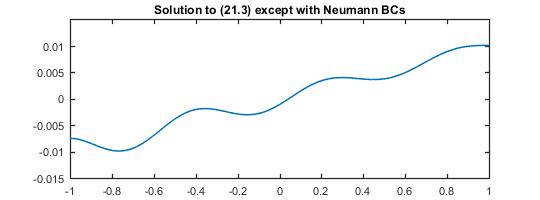
\includegraphics [width=4in]{chap21_05.png}
\begin{par}
 \vskip 1pt 
\end{par} \vspace{1em}
\begin{par}
Spectral methods can also solve problems with variable coefficients. For example, suppose we wish to solve the Airy equation boundary value problem $$ u'' - xu = 0, \quad u(-30) = 1, ~u(30) = 0 \eqno (21.4) $$ for $x\in [-30,30]$.  Here is the solution:
\end{par} \vspace{1em}
\begin{par}
 \vskip -2em 
\end{par} \vspace{1em}
\begin{verbatim}
L = chebop(@(x,u) diff(u,2)-x.*u,[-30,30]);
L.lbc = 1; L.rbc = 0; u = L\0;
plot(u), title('Solution to Airy equation (21.4)',FS,9)
\end{verbatim}

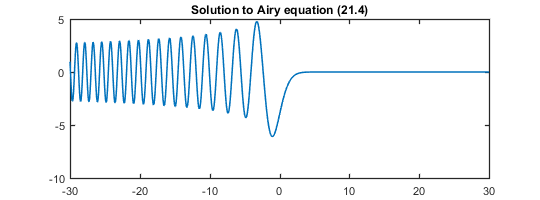
\includegraphics [width=4in]{chap21_06.png}
\begin{par}
 \vskip 1pt 
\end{par} \vspace{1em}
\begin{par}
For nonlinear problems, one would normally use a Newton iteration or some variant. Chebfun handles these cases too.  For example, the equation $$ \theta'' + \sin(\theta) = 0, \quad \theta\in [0,6]  \eqno (21.5a) $$ describes the motion in time of a nonlinear pendulum situated at height $h(t) = -\cos(\theta(t)) \in [-1,1]$. If we prescribe boundary conditions $$ u(0) = -\pi/2, \quad u(6) = \pi/2, \eqno (21.5b) $$ we can solve the system numerically with Chebfun as follows. Notice that the solution is still invoked by the backslash command, though we are very far now from the original Matlab notion of backslash for solving a square system of linear equations.
\end{par} \vspace{1em}
\begin{par}
 \vskip -2em 
\end{par} \vspace{1em}
\begin{verbatim}
N = chebop(0,6);
N.op = @(theta) diff(theta,2) + sin(theta);
N.lbc = -pi/2; N.rbc = pi/2; theta = N\0;
plot(-cos(theta)), grid on, ylim([-1 1])
title('Nonlinear pendulum (21.5)',FS,9)
xlabel('t',FS,10), ylabel('height -cos(\theta)')
\end{verbatim}

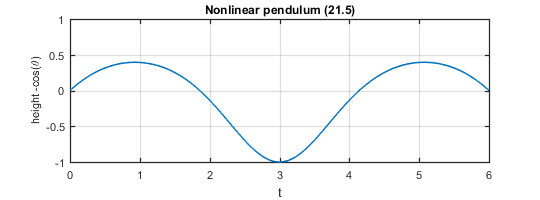
\includegraphics [width=4in]{chap21_07.png}
\begin{par}
 \vskip 1pt 
\end{par} \vspace{1em}
\begin{par}
This solution corresponds to the pendulum first going up above height 0 for a time, then swinging over to the other side, where it again goes above height 0 before falling back down again. On the other hand, suppose we change the right-hand boundary condition to $5\pi/2$.  Then another solution appears, corresponding to the pendulum swinging once around the top:
\end{par} \vspace{1em}
\begin{par}
 \vskip -2em 
\end{par} \vspace{1em}
\begin{verbatim}
N.lbc = -pi/2; N.rbc = 5*pi/2; theta = N\0;
plot(-cos(theta)), grid on, ylim([-1 1])
title('Nonlinear pendulum (21.5), another solution',FS,9)
xlabel('t',FS,10), ylabel('height -cos(\theta)')
\end{verbatim}

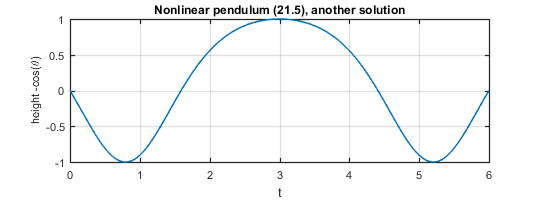
\includegraphics [width=4in]{chap21_08.png}
\begin{par}
 \vskip -4pt 
\end{par} \vspace{1em}
\begin{par}
These two solutions do not exhaust the full set of possibilities for this nonlinear problem; see Exercise 21.7.
\end{par} \vspace{1em}
\begin{par}

To compute solutions of nonlinear differential equations, Chebfun uses
variants of Newton's method implemented for continuous functions rather
than discrete vectors.  Where one might expect to encounter Jacobian
matrices in the solution process, Chebfun actually utilizes their continuous
analogues known as Fr\'echet derivative operators, which are constructed
by a process of automatic differentiation, again exploiting lazy
evaluation. These capabilities are due to Birkisson and Driscoll [2012].
Chebfun can also solve systems of equations, eigenvalue problems, and
problems specified by coefficients that are just piecewise smooth.

\end{par} \vspace{1em}
\begin{par}
This is a book about approximation theory, not differential equations, and we began this chapter with an approximation result, a theorem about the $O(\kern.7pt\rho^{-n})$ accuracy of derivatives of approximations of analytic functions.  It would be excellent if this theorem implied that spectral methods converge to analytic solutions at the rate $O(\kern.7pt\rho^{-n})$, but it does not. Theorem 21.1 ensures that if $u$ is an analytic solution to a boundary value problem $Lu = f$, then the Chebyshev interpolants to $Lu$ would converge geometrically to $f$ as $n\to\infty$.  In spectral computations, however, we do not have the exact solution available to discretize, but must approximate it by solving matrix problems.  One can hope that the approximations will converge at the expected rate, and indeed they do so under many circumstances, but proving this requires further arguments, which we shall not attempt to discuss here. As a rule, in this business, the practice is ahead of the theory.
\end{par} \vspace{1em}
\begin{par}
Some of the ideas behind spectral methods are as old as Fourier and Chebyshev expansions, and many people contributed in the early years of computers, including Lanczos, Elliott, Fox, and Clenshaw. But it was their application to the partial differential equations of fluid mechanics by Orszag and Gottlieb and others beginning around 1970 that made these methods famous, and it was Orszag who coined the term ``spectral methods'' [Orszag 1971a \& 1971b]. Spectral methods divide into Fourier methods, for periodic problems, and Chebyshev and related methods, for nonperiodic problems.  As always in this book, we have emphasized the nonperiodic case, which is less obvious, even though at bottom it is essentially the same. In applications, Fourier and Chebyshev discretizations are often found mixed together.  For example, a 3D cylindrical geometry may be discretized by a Chebyshev grid for the radial variable, a periodic Fourier grid for the circumferential variable, and another periodic grid serving as an approximation to an ideal infinite Fourier grid for the longitudinal variable.  When the grids are fine, implementations are often based on the Fast Fourier Transform rather than matrices.
\end{par} \vspace{1em}
\begin{par}
For details of the spectral methods incorporated in Chebfun, see [Driscoll, Bornemann \& Trefethen 2008] and [Driscoll \& Hale 2012] for the linear case and [Birkisson \& Driscoll 2012] for nonlinear aspects. For information about spectral methods in general, see texts such as [Fornberg 1996], [Trefethen 2000], [Boyd 2001], [Canuto, Hussaini, Quarteroni \& Zang 2006], [Hesthaven, Gottlieb \& Gottlieb 2007], and [Shen, Tang \& Wang 2011].
\end{par} \vspace{1em}
\begin{par}
This chapter began by noting that if a function is smooth, the derivatives of its interpolants converge rapidly. A contrapositive of this observation is the phenomenon that if the discrete approximations to derivatives of a function blow up as the mesh is refined, it is not smooth.  Chebfun exploits this principle as the basis of its edge detection algorithm for breaking piecewise smooth functions into subintervals, which was illustrated at the end of Chapter 9. This algorithm was developed by Rodrigo Platte and is described in $\hbox{[Pach\'on,}$ Platte \& Trefethen 2010].
\end{par} \vspace{1em}
\begin{par}

\begin{displaymath}
\framebox[4.7in][c]{\parbox{4.5in}{\vspace{2pt}\sl
{\sc Summary of Chapter 21.}
Spectral collocation methods are numerical algorithms for solving
differential equations based on polynomial or trigonometric interpolants.
For problems whose solutions are analytic, they typically converge
geometrically as the grid is refined.\vspace{2pt}}}
\end{displaymath}

\end{par} \vspace{1em}
\begin{par}
 \small\smallskip\parskip=2pt
\par
{\bf Exercise 21.1.  Proof of Theorem 21.1.}  Write down a careful
proof of Theorem 21.1
as a corollary of Theorems 3.1 and 8.1.  Be sure to state
precisely what properties of the Chebyshev polynomials
$\{T_k\}$ your proof depends on.
\par
{\bf Exercise 21.2.  Extension of Theorem 21.1.}  Theorem 21.1
quantifies the accuracy of the derivatives of Chebyshev interpolants
based on an assumption of analyticity in a Bernstein ellipse.
State and prove
a different theorem about the convergence of the derivatives for
{\em any\/} sequence of polynomials $p_n\in {\cal P}_n$ for which
the errors satisfy $\|f-p_n\| = O(\kern .7pt \rho^{-n})$ for
some $\rho > 1$.
\par
{\bf Exercise 21.3.  Differentiation matrices.}
(a) The text displayed the $3\times 3$ matrix $D(3)$.
Derive the entries of this matrix analytically.
(b) Also displayed was the $5\times 5$ matrix $D2(5)$.
Derive the entries of the middle column of this matrix analytically.
\par
{\bf Exercise 21.4.  Linear boundary value problems.}
Solve the following linear ODE boundary value problems
numerically with Chebfun.  In each case plot the solution and report
the value of $u$ at the midpoint of the interval and the length
of the chebfun representing $u$.
\hfill\break
(a) $0.001 u'' + x u' - u = \exp(-10x^2)$, $x\in[-1,1]$, $u(-1)=2$, $u(1)=1$.
\hfill\break
(b) $0.001 u'' + (1-x^2)u = 1$, $x\in[-5,5]$, $u(-5)=0$, $u(5)=0$.
\hfill\break
(c) $0.001u'' + \sin(x) u = 1$, $x\in[-10,10]$, $u(-10)=0$, $u'(10)=0$.
\par
{\bf Exercise 21.5.  Nonlinear boundary value problems.}
Find a solution numerically to each of the following nonlinear
ODE boundary value problems.
In each case plot the solution and report
the value of $u$ at the midpoint of the interval.
\hfill\break
(a) $0.05 u'' + (u')^2 - u = 1$, $x\in[0,1]$, $u(0)=2$, $u(1)=1$.
\hfill\break
(b) $0.01 u'' - u u' - u = 0$, $x\in[-1,1]$, $u(-1)=1$, $u(1)=2$.
\par
{\bf Exercise 21.6.  Convergence with \boldmath $n$.}
The text solved the boundary value problem $u''+u'+100u=x$
on $[-1,1]$ with boundary conditions
$u(-1) = u(1) = 0$ for grid parameters $n+1 = 5$, $12$, and $35$.
Perform a numerical study of the $\infty$-norm error of the
solution as a function of $n$, and comment on the results.
\par
{\bf Exercise 21.7.  Nonunique solutions.}
(a) For each of the two nonlinear pendulum problems solved at the end of
the chapter, determine exactly how many solutions there
must be.  (You can use physical reasoning, or phase plane analysis.)
(b) Find them all numerically with Chebfun by using
sufficiently close initial guesses specified by a command
of the form \verb|N.init = f(theta)| to start the iteration.  Report the
maximum heights ${-}\cos(\theta)$ of the pendulum in all cases, and the
time(s) at which these heights are reached.
\par
{\bf Exercise 21.8.  Painlev\'e equation.}  Solutions
to the second Painlev\'e equation, $u^{\prime \prime} = 2u^3+xu$,
typically blow up at various locations on the $x$-axis.
There exist special solutions, however, that are smooth
for all real $x$.   Characterized
by the asymptotic boundary conditions
$u \sim \pm \sqrt{-x/2}$ as $x \to -\infty$ and $u\to 0$ as $x\to+\infty$,
these are the so-called Hastings--McLeod solutions.
Truncate the problem to the interval $[-L,L]$ with boundary conditions
$u(-L) = \sqrt{L/2}$, $u(L)=0$ and compute and plot solutions for
$L = 1,2,4,8,16$.  Produce a table of $u(0)$ and $u'(0)$ for each value
of $L$.  To ten digits, what do you think are the values of
$u(0)$ and $u'(0)$ in the limit $L\to\infty\kern 1pt?$
\par
{\bf Exercise 21.9.  Formula for square differentiation matrix.}
Derive (21.2) from (5.8).

\end{par} \vspace{1em}



\end{document}
    
